\section{Statistical analysis}
\label{research-design-and-methodology:statistical-analysis}

The workloads of Section~\ref{research-design-and-methodology:workloads} and the metrics of Section~\ref{research-design-and-methodology:metrics-and-cost-model:cost-model} fix what is measured and how each sample is obtained. This section fixes the inference applied to those samples once collected. The analysis pipeline is specified in advance rather than chosen after inspecting the data, and it follows the reporting discipline surveyed in Section~\ref{related-work:benchmarking-methodology-for-data-systems}. Accordingly, the benchmarking framework persists every raw iteration (Section~\ref{system-architecture-and-implementation:measurement-instrumentation-and-cost-model}), while the analysis reduces the resulting distributions to defensible findings. The unit of analysis throughout is a single per-iteration sample, comprising elapsed time, bytes received, bytes sent, and the cost derived from them, keyed by the tuple of configuration, workload, dataset tier, and benchmark run. Figure~\ref{fig:statistical-analysis-pipeline} traces this pipeline from the per-iteration sample through estimator selection, uncertainty quantification, and pairwise comparison to the three research questions, where \acrshort{rq}3 consumes the outputs produced for \acrshort{rq}1 and \acrshort{rq}2. Each question is then answered in turn: \acrshort{rq}1 in Section~\ref{research-design-and-methodology:statistical-analysis:answering-rq1-cloud-native-vs-traditional}, \acrshort{rq}2 in Section~\ref{research-design-and-methodology:statistical-analysis:answering-rq2-scaling-against-single-node}, and \acrshort{rq}3 in Section~\ref{research-design-and-methodology:statistical-analysis:answering-rq3-consistency-across-patterns}.

\begin{figure}[H]
	\centering
	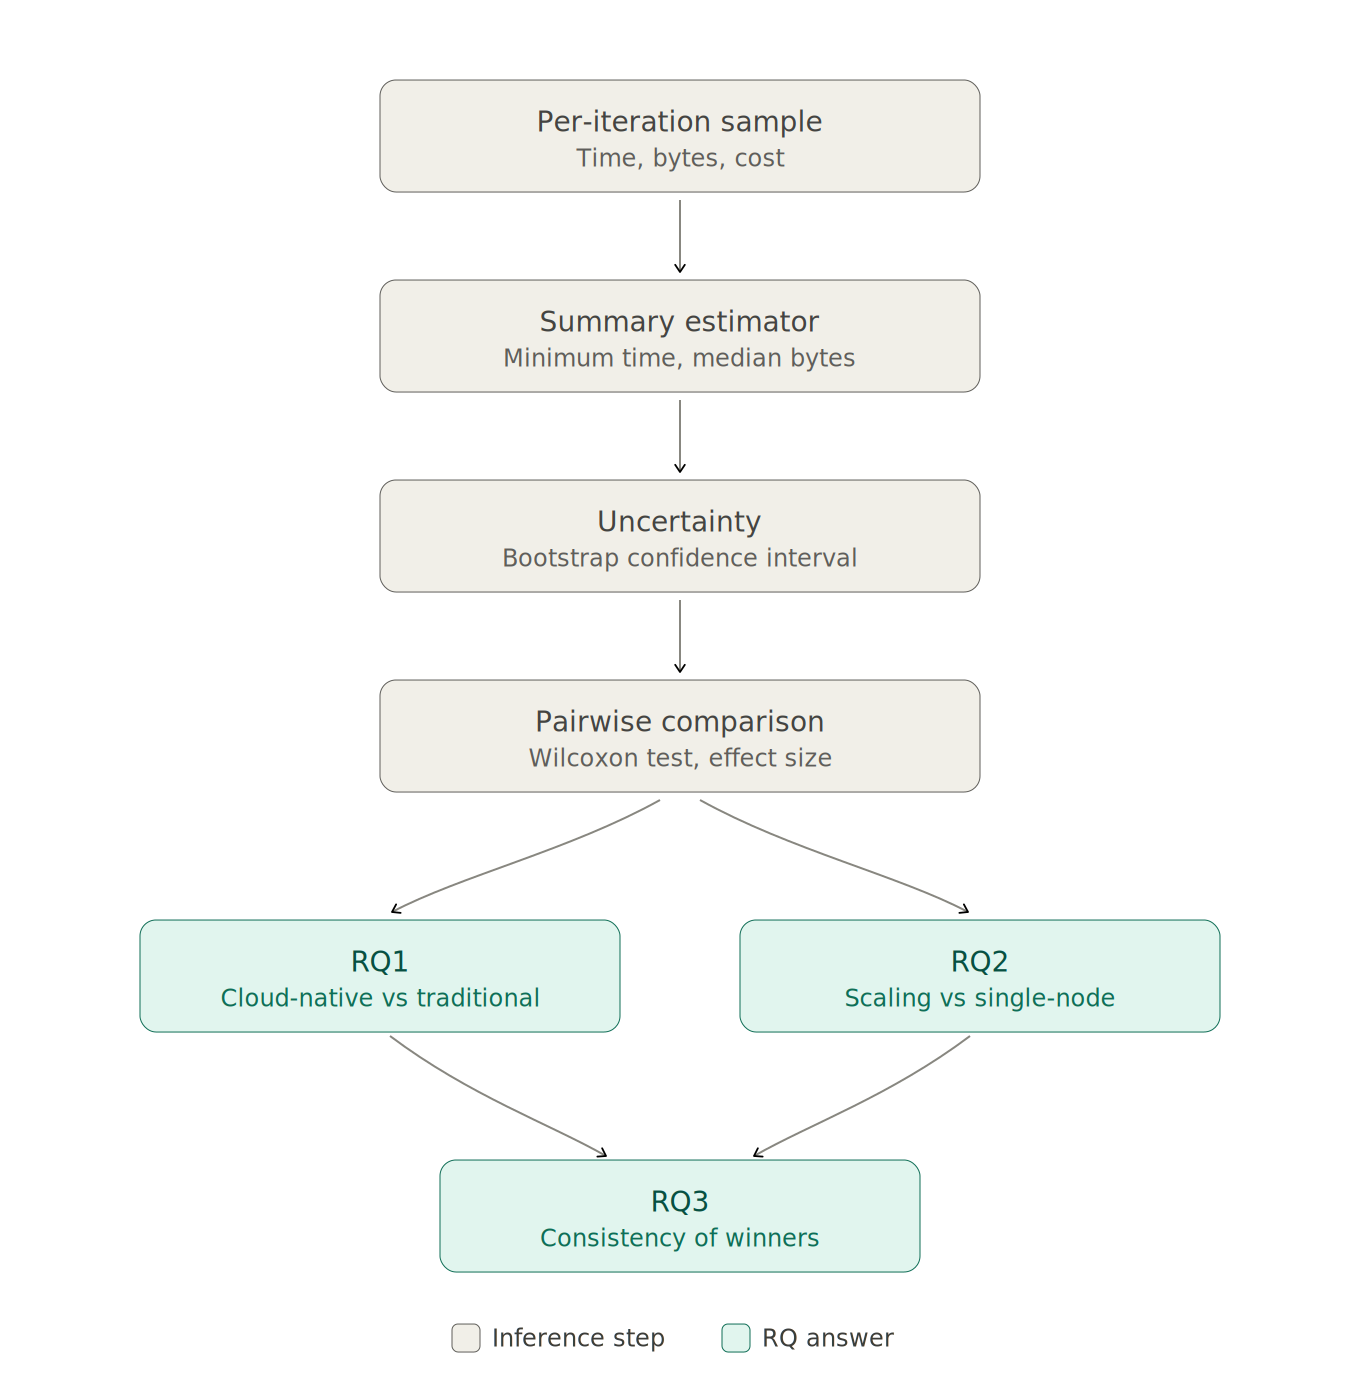
\includegraphics[width=0.7\textwidth]{Chapters/04-research-design-and-methodology/sub-chapters/figures/04-statistical-analysis-pipeline.png}
	\caption[Statistical analysis pipeline]{The statistical analysis pipeline, from a per-iteration sample through the summary estimator, uncertainty quantification, and pairwise comparison to the three research questions. RQ1 and RQ2 are answered from the pairwise stage, and RQ3 consumes their outputs.}
	\label{fig:statistical-analysis-pipeline}
\end{figure}

\subsection{Measurement-quality terminology}
\label{research-design-and-methodology:statistical-analysis:measurement-quality-terminology}
Every claim this chapter makes about the quality of a measured number rests on the metrology vocabulary standardized by \textcite{jcgm2012_international_vocabulary_of_metrology}. That vocabulary separates accuracy, the closeness of a measurement to the true value, from precision, the closeness of repeated measurements to one another, and it distinguishes repeatability from reproducibility by which conditions are held constant between measurements. Two such conditions structure the present design. Repeatability here refers to variation across the timed iterations of a single warm engine, where configuration, host, and input are fixed and only uncontrolled run-to-run noise remains. Reproducibility refers to variation across the seeded re-runs described in Section~\ref{research-design-and-methodology:overview-and-experimental-design:replication-and-randomization}, where the entire measurement is repeated under nominally identical but separately provisioned conditions. The confidence intervals reported in Section~\ref{research-design-and-methodology:statistical-analysis:uncertainty-quantification} quantify repeatability; reproducibility is probed separately by comparing the seeded re-runs, and because it holds only the nominal configuration fixed rather than the host and input as well, it is the wider of the two. Table~\ref{tab:repeatability-vs-reproducibility} sets the two conditions side by side along these axes.

\begin{table}[H]
	\centering
	\begin{tabular}{@{}l >{\raggedright\arraybackslash}p{0.23\textwidth} >{\raggedright\arraybackslash}p{0.17\textwidth} >{\raggedright\arraybackslash}p{0.21\textwidth} @{}}
		\toprule
		Condition & What varies & Held constant & Quantified by \\
		\midrule
		Repeatability & Run-to-run noise across timed iterations & Configuration, host, input & Confidence interval (\S~\ref{research-design-and-methodology:statistical-analysis:uncertainty-quantification}) \\
		Reproducibility & Full re-measurement under separate provisioning & Nominal configuration only & Seeded re-runs (\S~\ref{research-design-and-methodology:overview-and-experimental-design:replication-and-randomization}) \\
		\bottomrule
	\end{tabular}
	\caption[Repeatability versus reproducibility]{The two measurement conditions distinguished in this design, the source of variation each admits, what is held fixed, and the analysis that quantifies it. Reproducibility is the wider of the two.}
	\label{tab:repeatability-vs-reproducibility}
\end{table}

\subsection{Summary statistics and the choice of estimator}
\label{research-design-and-methodology:statistical-analysis:summary-statistics-and-the-choice-of-estimator}

Wall-clock time is bounded below, and its contamination runs in one direction only: a query cannot execute faster than its work allows, whereas scheduling delays, resource contention, and garbage-collection pauses can only add time. The true cost of a query is therefore approached from above, and the fastest observed iteration lies closest to it. The minimum over repeated short runs is consequently adopted as the location summary for elapsed time, in preference to the mean or the median, both of which are pulled upward by the same contamination the minimum rejects \parencite{chen2016_robust_benchmarking_noisy_environments}. Figure~\ref{fig:estimator-one-sided-contamination} shows this geometry. One-sided contamination produces a right-skewed distribution with a hard lower bound: the minimum lies nearest the true value, while the mean and the median are drawn into the longer elapsed times of the contamination tail. This reasoning does not carry over to the transfer metrics. Bytes received and bytes sent are not lower-bounded noise in the same sense, since a configuration has no single true byte count that observations only ever exceed, and their run-to-run variation reflects genuine differences in what was read or returned. They are therefore summarized by the median, with the full distribution retained for inspection rather than reduced to a single number. Cost is a deterministic function of duration and allocated resources rather than an independently measured quantity, so its summary inherits the estimator applied to duration rather than being computed from a distribution of its own.

\begin{figure}[H]
	\centering
	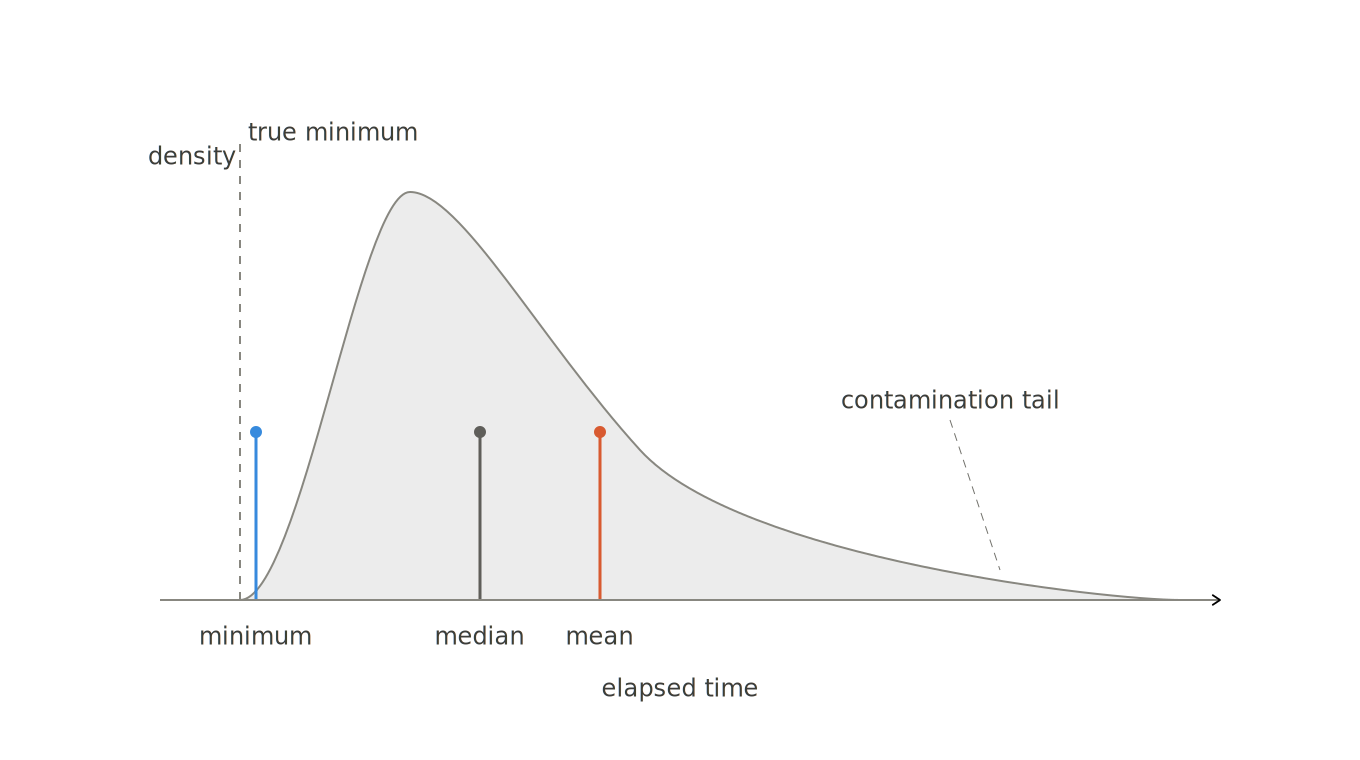
\includegraphics[width=0.9\textwidth]{Chapters/04-research-design-and-methodology/sub-chapters/figures/04-estimator-one-sided-contamination.png}
	\caption[Estimator choice under one-sided contamination]{Estimator choice for a one-sidedly contaminated timing distribution. The hard left bound is the true minimum; the minimum estimator lies nearest it, while the median and the mean are pulled rightward into longer elapsed times by the contamination tail.}
	\label{fig:estimator-one-sided-contamination}
\end{figure}

\subsection{Uncertainty quantification}
\label{research-design-and-methodology:statistical-analysis:uncertainty-quantification}

\textcite{hoefler2015_scientific_benchmarking_parallel} argues for reporting a metric as its distribution rather than as a single point average. Each metric is therefore reported primarily as a distribution, so a configuration's spread is visible alongside its central tendency. A bootstrap attaches an interval to each summary. The per-iteration samples for a given configuration and workload are resampled with replacement, and the confidence interval is read from the resulting sampling distribution of the estimator. The interval quantifies within-engine repeatability, as defined in Section~\ref{research-design-and-methodology:statistical-analysis:measurement-quality-terminology}, not reproducibility. The seeded re-runs probe reproducibility instead. Cloud performance variability documented in Section~\ref{related-work:benchmarking-methodology-for-data-systems} widens these intervals, and that widening is treated as a measured property of running on shared cloud infrastructure rather than as an error to be suppressed.

\subsection{Pairwise comparison and effect size}
\label{research-design-and-methodology:statistical-analysis:pairwise-comparison-and-effect-size}
The analysis does not assume that the measured distributions are normal. Two configurations evaluated on the same workload are compared with the Wilcoxon rank-sum test applied to their paired samples. The pairing follows the concurrent same-window execution established in Section~\ref{research-design-and-methodology:overview-and-experimental-design:replication-and-randomization}. \textcite{laaber2019_software_microbenchmarking_cloud} show that running test and control on the same instance in randomized order, then comparing them with this test, reliably detects slowdowns of ten percent or less under cloud variability. A significant result is necessary but not sufficient, because significance reports only whether a difference exists, not how large it is. Each test is therefore reported with the Vargha--Delaney $\hat{A}_{12}$ effect size, with values near $0.5$ read as no effect and $0.56$, $0.64$, and $0.71$ marking the small, medium, and large thresholds \parencite{arcuri2014_hitchhiker_statistical_tests}. Table~\ref{tab:vargha-delaney-thresholds} summarizes these thresholds. The design issues several pairwise tests across configurations, workloads, and dimensions. Each result therefore states the number of tests in its family and whether a correction for multiple comparisons is applied, keeping the family-wise reading honest.

\begin{table}[H]
	\centering
	\begin{tabular}{@{}rl@{}}
		\toprule
		$\hat{A}_{12}$ & Effect size \\
		\midrule
		$0.50$ & Negligible \\
		$0.56$ & Small \\
		$0.64$ & Medium \\
		$0.71$ & Large \\
		\bottomrule
	\end{tabular}
	\caption[Vargha--Delaney effect-size thresholds]{Interpretation thresholds for the Vargha--Delaney $\hat{A}_{12}$ effect size. Values near $0.5$ indicate no effect; the listed thresholds mark the lower bound of each magnitude band. Adapted from \parencite{arcuri2014_hitchhiker_statistical_tests}.}
	\label{tab:vargha-delaney-thresholds}
\end{table}

\subsection{Answering RQ1: Cloud-native vs. traditional}
\label{research-design-and-methodology:statistical-analysis:answering-rq1-cloud-native-vs-traditional}

\acrshort{rq}1 is addressed by comparing the three single-node configurations, DuckDB over GeoParquet, PostGIS, and DuckDB over Shapefile, with the pairwise procedure of Section~\ref{research-design-and-methodology:statistical-analysis:pairwise-comparison-and-effect-size}, applied separately for each query pattern and each dataset tier across all three outcome dimensions of time, bytes, and cost. The access-pattern divide established in Section~\ref{background:spatial-data-formats-and-storage-models:summary} frames the interpretation: formats that a client can read in part through range requests and formats that require a full scan are expected to separate first on bytes received, and only afterward, if at all, on elapsed time. The byte comparison is therefore read as the more direct expression of the format difference, and the time comparison as its downstream consequence. The Shapefile configuration is treated asymmetrically because it is evaluated at the small tier only: every comparison involving Shapefile is reported at that tier and never extrapolated to the larger one, and a ranking that includes Shapefile is read as valid only where all three configurations were measured.

\subsection{Answering RQ2: Scaling against single-node}
\label{research-design-and-methodology:statistical-analysis:answering-rq2-scaling-against-single-node}
\acrshort{rq}2 is answered by tracing how the national-scale spatial join scales with parallelism. Speedup and parallel efficiency are computed as functions of worker count across the levels 2, 4, 8, 12, and 16 nodes. Each Sedona execution strategy is treated separately, with the default strategy as the baseline against which broadcast and partitioned execution are read. For a configuration run on \(n\) workers with per-tier elapsed time \(T_n\) under the minimum estimator of Section~\ref{research-design-and-methodology:statistical-analysis:summary-statistics-and-the-choice-of-estimator}, speedup \(S(n)\) and parallel efficiency \(E(n)\) are defined in Equation~\ref{eq:speedup-parallel-efficiency} relative to the smallest tested cluster of \(n_0 = 2\) nodes; ideal linear scaling then yields \(E(n) = 1\). Sub-linear scaling, where doubling the worker count fails to halve the run-time, is interpreted against the coordination-overhead argument of Section~\ref{background:cloud-native-data-architecture:distributed-and-non-distributed-computation} and the spatial-skew failure mode of Section~\ref{background:distributed-spatial-processing:spatial-partitioning-and-parallel-efficiency}, so that a flat or worsening curve is attributed to a named mechanism rather than left as an unexplained absence of speedup.

\begin{equation}
	S(n) = \frac{T_{n_0}}{T_n}, \qquad E(n) = \frac{n_0}{n}\,S(n), \qquad n_0 = 2
	\label{eq:speedup-parallel-efficiency}
\end{equation}

The comparison against the single-node engines is framed as a hardware-cost question after \textcite{mcsherry2015_scalability_but_at_what_cost}. The analysis locates the worker count, if any, at which a distributed configuration first overtakes the best single-node engine on a given workload and dimension, and reports whether such a crossover is observed within the tested range of 2 to 16 workers or only bounded below by it. To attribute scaling behavior to a specific part of the distributed lifecycle rather than to the bare label of distribution, the distributed wall-clock time is decomposed into the phase metrics of Section~\ref{research-design-and-methodology:metrics-and-cost-model:distributed-phase-metrics}, separating executor read time, shuffle volume, and driver collection. A failure to scale can then be traced to a costly shuffle or a large collection. The warm-cluster measurements do not satisfy the independence that the single-node samples approximate, because autoscaling and the exclusion of the provisioning interval from the timed window introduce structure into the run-to-run variation. These are discussed as identified sources of variance rather than averaged away as if the runs were exchangeable.

\subsection{Answering RQ3: Consistency across patterns}
\label{research-design-and-methodology:statistical-analysis:answering-rq3-consistency-across-patterns}

\acrshort{rq}3 is an analysis question rather than a separate measurement. It asks whether the configuration that performs best under \acrshort{rq}1 holds that position across every query pattern and all three outcome dimensions, or whether the best choice changes from one pattern or dimension to another. The analysis answers it by ranking the configurations within each pair of workload and outcome dimension, drawing on the effect sizes of Section~\ref{research-design-and-methodology:statistical-analysis:pairwise-comparison-and-effect-size} to decide when a difference in rank reflects a real separation rather than measurement noise. Rank stability and rank inversion are reported explicitly. A configuration that wins on elapsed time but loses on cost, or that leads on one query pattern and trails on another, is the kind of finding \acrshort{rq}3 exists to surface, so the ranking keeps such inversions visible rather than folding them into a single aggregate verdict. The subsection consumes the test outputs produced for \acrshort{rq}1 in Section~\ref{research-design-and-methodology:statistical-analysis:answering-rq1-cloud-native-vs-traditional} and for \acrshort{rq}2 in Section~\ref{research-design-and-methodology:statistical-analysis:answering-rq2-scaling-against-single-node}, and introduces no new statistical test of its own.